\documentclass[tikz,border=5pt]{standalone}
\usepackage{newtxmath}
\begin{document}

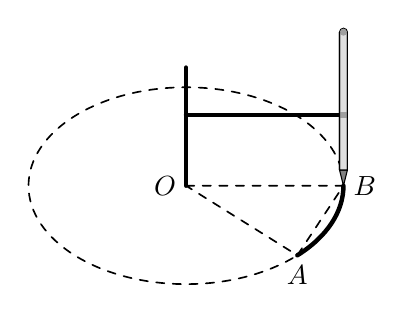
\begin{tikzpicture}[line cap=round,line join=round]
\coordinate (O) at (0,0);
\coordinate (B) at (2,0);
\coordinate (A) at (-45:2cm and 1.25cm);
\draw[dashed,semithick] (O) ellipse [x radius=2cm,y radius=1.25cm];
\draw[ultra thick] (B) arc[start angle=0,end angle=-45,x radius=2cm,y radius=1.25cm];
\draw[dashed,semithick] (O) node[left] {$O$} -- (B) node[right] {$B$} -- (A) node[below] {$A$} --cycle;

\draw[ultra thick] (O) -- ++(up:1.5) (up:0.9) -- ++(2,0) coordinate (tmp);
\path[draw=black,fill=gray] (B) -- ++(.05,.2) coordinate(B1) -- ++(-.1,0) coordinate(B2) -- cycle;
\path[draw=black,fill=gray!25] (B1) -- ++(0,1.75) coordinate (C1) arc[start angle=0,end angle=180,radius=0.05] coordinate (C2) -- (B2) -- cycle;
\draw[line width=2pt,gray!75,line cap=butt] ([xshift=-.05cm]tmp) --++(.1,0);
\fill[gray!75] ([xshift=-.05cm]C1) circle[radius=.045];
\draw (B1) -- (C1) (B2) -- (C2);
\end{tikzpicture}

\end{document}